\section{Livelits by Example}\label{sec:case-studies}


In this section, we will detail the livelits mechanism by way of  
two domain-specific case studies:
a course grade assignment case study in Sec.~\ref{sec:live-grading}
and an image transformation case study in Sec.~\ref{sec:image-transformation}.
% We also briefly mention several other examples in Sec.~\ref{sec:additional-examples}.\todo{do we?}{}
These case studies have been implemented
in Hazel, a browser-based live programming environment for a dialect of Elm. 
Elm is an industrial pure typed functional language in the
ML family used for client-side web development. 
We assume basic familiarity with ML.

\subsection{Case Study: Grading with Livelits}\label{sec:live-grading}
Consider this familiar scenario: an instructor needs
(1) to record numeric grades for various assignments and exams, and
(2) to visualize and perform various computations with these numeric grades
in order ultimately to assign final letter grades.
(In fact, this case study is not contrived: one author is using Hazel to compute grades this semester.)

The most common end-user application for this task is the spreadsheet, because 
it allows the instructor to record grades using a natural tabular interface,
visualize this data in one of a finite number of plot styles, 
and perform basic computations,
with results updated live.
However, these affordances are limited. 
It is difficult to package up common operations 
into reusable libraries, interact with the data using domain-specific visualizations,
and perform complex, unanticipated operations 
(e.g. preparing the data in an idiosyncratic format demanded by the university's grading system).

General-purpose programming languages 
can handle these scenarios, but users 
lose the ability to receive live feedback and  
directly manipulate data and visualizations in the editor.

Livelits are able to address this tension.
Fig.~\ref{fig:grading}(c)\todo{sublabels} shows a Hazel program where 
the instructor alternates between programmatic and direct manipulation in several situations.

First, the instructor defines a value \li{grades} 
that records the grades for each student using a livelit, \li{\$dataframe}, 
that implements a tabular user interface. The formula bar 
allows the selected cell to be filled with an arbitrary Hazel expression, 
with all of Hazel's editor services available. 
For the sake of demonstration, we show a cell that has been filled using another livelit, 
\li{\$slider}, in combination with symbolic manipulation.\todo{do this?}{}
The table itself displays not the expression itself but rather its value, just as in a spreadsheet.

Next, the instructor programmatically computes the overall \li{averages} 
for each student by applying \li{compute_averages}, a helper function 
defined in the usual way in a library  (not shown) shared between multiple courses.

Next, the instructor wants to ``eyeball'' reasonable \li{cutoffs} between letter grades 
by directly manipulating a highly domain-specific livelit, \li{\$cutoffs}, that provides draggable ``paddles'' 
superimposed on a live visualization of the distribution of the \li{averages} value provided as a parameter 
(for the sake of space, we plot dots rather than a histogram).
% The value of \li{cutoffs} is a labeled 4-tuple containing each cut-off. 

Finally, 
the instructor programmatically assigns letter grades to each student 
based on the selected \li{cutoffs} 
by calling \li{assign_grades} 
and formats these for submission with \li{format_for_university},
again shared functions.

\subsubsection{Livelit Expansion}\label{sec:livelit-expansion}
Livelit expressions are given dynamic meaning by expansion to core expressions, which do not contain livelits.
For example, the expansion of Fig.~\ref{fig:grading} is:

\begin{lstlisting}[xleftmargin=0.2cm]
let grades = Dataframe (
  ["A1", "A2", "A3", "Midterm", "Final"],
  [("Alice", [24. +. 36. +. 33., 
               92., 83.5, 95., 88.]),
   ("Bob", [61., 64., 98., 70., 85.]),
   ("Ciri", [75., 81., 73., 82., 79.]),
   (* ... *) ]) in
let averages = compute_averages grades weights in
let cutoffs = (.A 90., .B 80., .C 70., .D 60.) in
format_for_university 
  (assign_grades averages cutoffs)
\end{lstlisting}

The programmer can inspect this expansion in Hazel.
Ideally, however, it would not be necessary to inspect the expansion
(or the livelit implementation, which specifies the expansion logic and is discussed in Sec.~\ref{sec:livelit-definitions})
to reason about types and binding.
After all, one does not need to look inside
function bodies to reason about types and binding.
Instead, in the words of \citet{DBLP:conf/ifip/Reynolds83},
``type structure is a syntactic discipline for maintaining levels of abstraction''.
The livelits mechanism supports reasoning abstractly about types and binding by
several means.

To support abstract reasoning about the type of the expansion,
livelit definitions declare an \emph{expansion type}.
The declarations of the two livelits in Fig.~\ref{fig:grading},
eliding their implementations, are:
\begin{lstlisting}[numbers=none]
livelit $dataframe at Dataframe { ... }
livelit $grade_cutoffs(avgs: List(Float))
  at (.A Float, .B Float, .C Float, .D Float) { ... }
\end{lstlisting}
The expansion type of \li{\$dataframe} is \li{Dataframe}
(a type classifying tabular floating point data together with string row and column keys, consistent with the expansion above)
and the expansion type of \li{\$grade_cutoffs} is a labeled product of grade cutoffs (Hazel notates labels \li{.label}).
Hazel summarizes the typing information from the livelit definition when the cursor is on the livelit's name,
just as it displays a function's type when its name is under the cursor (not shown).

\subsubsection{Typed Hygienic Splicing and Parameterization}\label{sec:splicing-and-parameterization}
Livelit expressions can include sub-expressions in one of two ways:
as parameters or as splices.

\paragraph{Parameters}\label{sec:parameterization} Parameters appear immediately after the name of the applied livelit.
For example, \li{averages} is provided as a parameter to \li{\$grade_cutoffs} in Fig.~\ref{fig:grading}.
The livelit declares a fixed number of parameters and specifies their types in its declaration.
For example, the declaration of \li{\$grade_cutoffs} shown above specifies one parameter of type \li{List(Float)}
(the grades data to be plotted, see below).

Livelit abbreviations can partially apply parameters. Consider the slider livelit
from Fig.~\ref{fig:color}:
\begin{lstlisting}[numbers=none]
livelit $slider (min: Float) (max: Float) at Float { ... }
\end{lstlisting}
We can partially apply the first parameter as follows to define a parameterized non-negative slider livelit with one remaining parameter:
\begin{lstlisting}[numbers=none]
livelit $nnslider = $slider 0.0 in ...
\end{lstlisting}
Only livelits with no remaining parameters can be used to fill a hole.
So writing \li{\$nnslider} in expression position will not display the slider GUI. Instead, it will display as a ``missing livelit parameter'' error.%
\footnote{\label{footnote:typing}In Hazel, erroneous expressions are automatically placed inside holes so that they do not prevent other parts of the program from executing
\cite{HazelnutLive}.}


\begin{figure*}
  \begin{center}
    \begin{subfigure}[t]{0.5\textwidth}
      \centering
      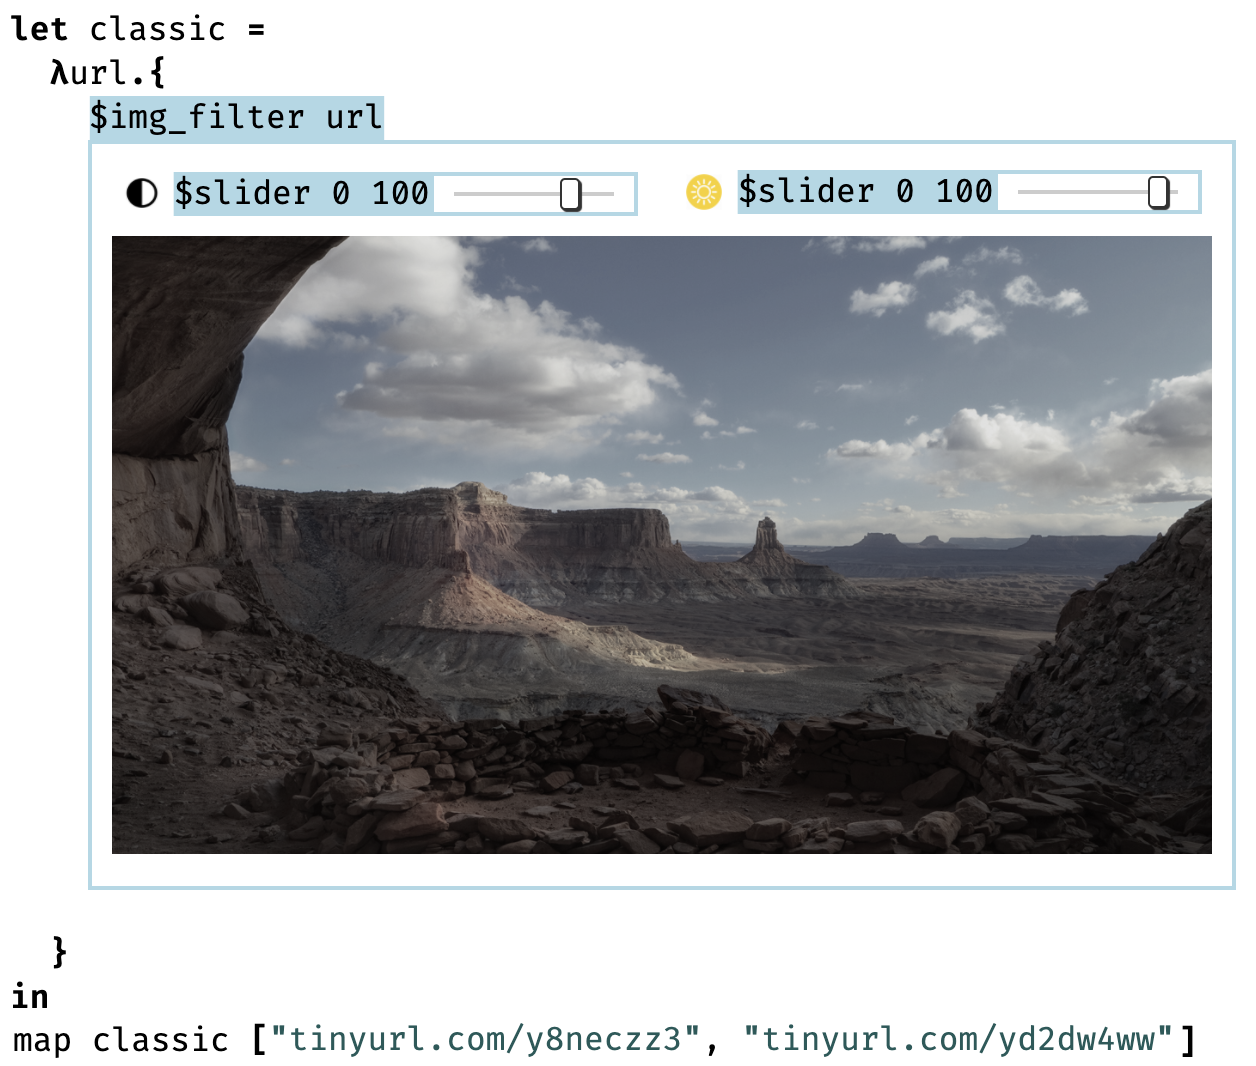
\includegraphics[width=15pc]{img-filter-1.png}
      \caption{}
    \end{subfigure}\begin{subfigure}[t]{0.5\textwidth}
      \centering
      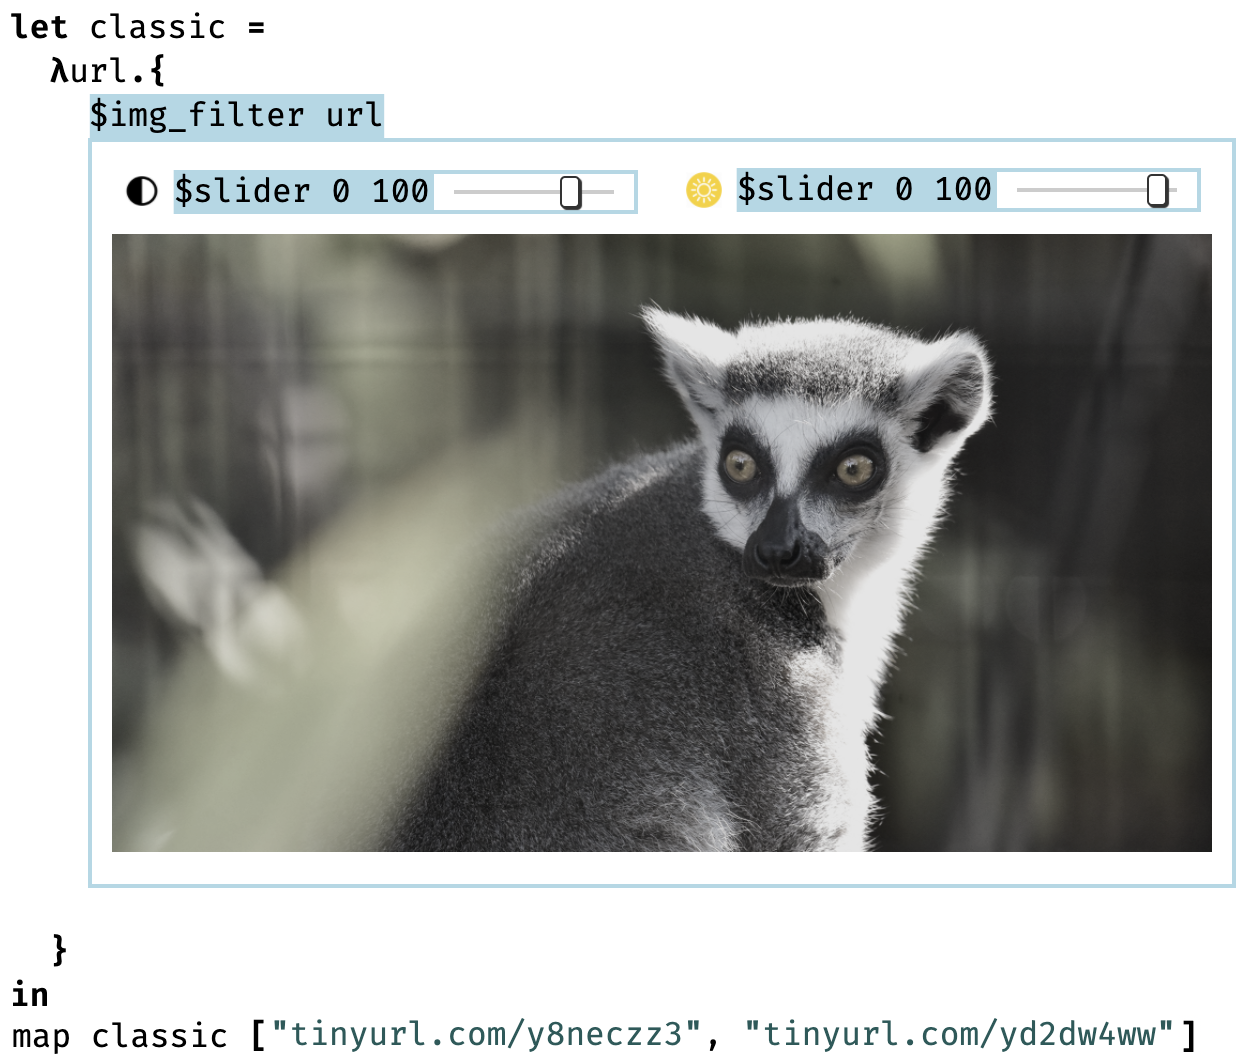
\includegraphics[width=15pc]{img-filter-2.png}
      \caption{}
    \end{subfigure}
  \end{center}
  \caption{Case Study: Image Transformation. The image shown is determined based on the selected closure.}
  \label{fig:img-transformation}
\end{figure*}


\paragraph{Splices}\label{sec:splices}
Spliced expressions (or \emph{splices}) appear directly inside the livelit GUI.
Splices can be filled with Hazel expressions of any form, including other livelit expressions,
and all of Hazel's editing affordances are available when editing these expressions.
For example, each cell in the \li{\$dataframe} GUI in Fig.~\ref{fig:grading}
has a corresponding splice, which appears in the formula bar at the top of the livelit
when the user has selected that cell.
The cell itself displays the live value of the spliced expression,
following the example of spreadsheet interfaces
(we return to live evaluation in Sec.~\ref{sec:live-evaluation} below).

The livelit provides an expected type for each splice.
For example, the splices for the row and column keys in Fig.~\ref{fig:grading} are expected to be expressions
of type \li{String}, and the remaining cells are expected to be expressions of type \li{Float}.
Hazel surfaces this typing information for the programmer when the cursor is in a splice,
so it is not necessary to inspect the expansion or the livelit implementation.
If an expression of invalid type is entered, it will display in an error hole as usual,
and in Hazel this will not prevent evaluation of other expressions (see Footnote \ref{footnote:typing}).

Unlike parameters, the number of splices is not fixed in the livelit declaration. Splices can be created,
deleted, and filled through user interaction with the livelit. For example, clicking the \li{+} buttons
in Fig.~\ref{fig:grading} will create new rows or columns, which will in turn generate new splices.

\paragraph{Hygiene}\label{sec:hygiene}
Parameters and splices can both appear in the expansion. For example,
the expansion of the \li{\$dataframe} livelit in Fig.~\ref{fig:grading} includes the
entered cell contents and the row and column keys.

The client cannot know, without looking at the expansion or the livelit implementation,
where in the expansion each parameter or splice will appear. This becomes relevant when
the expansion places the parameter or splice under a binder, e.g. in the body of a function or let binding.
Na\"ively, this could cause inadvertent capture of the bound variable by a free variable
in the parameter or splice. For example, consider a livelit that generates an expansion
of the following form:
\begin{lstlisting}[numbers=none]
let len = strlen <splice1> in
(<splice2>, <splice2> + 1)
\end{lstlisting}
Here, \li{<splice2>} appears under the binding of \li{len}. If the client's choice for
\li{<splice2>} itself refers to a client-side binding of the same identifier, \li{len},
it would na\"ively be captured. This sort of bug would difficult to debug,
both for the livelit provider and the client.

To avoid this situation, the livelit expansion mechanism
maintains parameter and splice hygiene: parameters and splices are included in the expansion
in a capture-avoiding manner.
Consequently, clients can reason abstractly about binding in splices: variables in splices
always refer to bindings visible to the client, rather than bindings that are hidden inside expansions.
% This is implemented by alpha-renaming bindings internal to the expansion as necessary.
% (We discuss potentially relaxed variations of this hygiene discipline in Sec.~\ref{sec:discussion}.)

\subsubsection{Live Evaluation}\label{sec:live-evaluation}
Livelits can request the result of evaluating a splice or a parameter.
For example, the \li{\$dataframe} livelit uses this facility to display
the evaluation result for each cell when the cursor is not on it, like a spreadsheet.
The \li{\$grade_cutoffs} livelit uses this facility to plot the grades list, provided
as a parameter, on the number line.

\paragraph{Closure Collection} Evaluation in Hazel is, as usual, defined only for closed expressions,
but parameters and splices can both refer to variables in the surrounding
context. In order to provide evaluation results for parameters or splices containing free variables,
Hazel performs \textbf{closure collection} in two phases.

In the first phase, Hazel evaluates the program after placing holes in place of each livelit,
following the evaluation semantics for incomplete programs developed by \citet{HazelnutLive}.
The result is an expression with holes in it, each of which is equipped with a closure.
For example, there is a single closure associated with the application of \li{\$dataframe} in Fig.~\ref{fig:grading}.
This closure contains the value of the \li{weights} variable from Line 1 and any other variables in the context
around that livelit, e.g.
from imported libraries, not shown. Consequently, when the livelit requests the evaluation result for
splices that use these variables, such as the cell shown selected in Fig.~\ref{fig:grading},
an evaluation result is available. (We consider the situation where more than one closure is available
in the Sec.~\ref{sec:image-transformation}.)

Similarly, the closure for the \li{\$grade_cutoffs} livelit in Fig.~\ref{fig:grading} includes a result for
the \li{grades} variable. However, this variable's result, along with the
results for other variables that depend on \li{grades}, such as \li{averages}, ultimately depend on the
expansion of the \li{\$dataframe} livelit. If we stop after the first phase of closure collection,
where these expansions have not yet been included,
then no useful result will be available here.
For this reason, there is a second phase of closure collection where any livelit holes that appear
in the collected livelit closures are \emph{resumed}, i.e. the expansion is generated
(in this case, for the \li{\$dataframe} livelit) and is used to fill
the hole before evaluation resumes, following the semantics for resumption developed by \citet{HazelnutLive}.
Livelit expansions do not themselves contain livelits, so no subsequent resumption phases are necessary.

The final evaluation result for the program as a whole can also proceed by resumption, because
closure collection performs all of the computations that do not ultimately depend on the livelit expansion.
Consequently, Hazel does not need to evaluate the program multiple times in order to support edit-time
(i.e. live) evaluation in this way.

\paragraph{Indeterminate Results}
We used the phrase \emph{evaluation result} rather than \emph{value} above purposefully:
splices and parameters can be incomplete, i.e. they can contain holes, so
evaluation does not always result in a value \cite{HazelnutLive}.
In particular, when a hole appears in elimination position, e.g. in function position of a function application,
 the result is instead an indeterminate expression.
When a livelit requests an evaluation result, it must be able to handle indeterminate results.
For example, if the parameter to \li{\$grade_cutoffs} were a hole or some other indeterminate expression,
then it would have degraded functionality
(in this case, it would display the list elements that are values on the timeline, skipping indeterminate elements).
We will return to how livelit implementations handle this situation in Sec.~\ref{sec:livelit-definitions}.



\subsection{Case Study: Image Transformations}\label{sec:image-transformation}

Our next case study is a simple image transformation livelit, \li{\$img_filter},
demonstrated in Fig.~\ref{fig:img-transformation}. This livelit takes 
a URL to an image as a parameter, and contains two splices of type \li{Int},
one to adjust the contrast, and the other to adjust the brightness.
In this example, we have filled those splices with a \li{\$slider}, but 
as above we could enter any expression of type \li{Int}.
The livelit shows a live preview of the transformed image.
The expansion generates the necessary calls to image processing functions, 
not shown.

The novelty in this example is that the livelit appears inside a function, 
\li{classic}, which takes an image URL as input. At the bottom 
of the figure, \li{classic} is mapped over a list (here, containing only 
two elements for the sake of presentation). Consequently, there are now 
two closures associated with the application of \li{\$img_filter} in the 
body of \li{classic}. Rather than disabling live evaluation in situations like 
this, Hazel instead allows the programmer to select between the closures when 
the cursor is on the livelit expression (via a simple sidebar toggle, not shown, which is shared 
with the general closure selection UI \cite{HazelnutLive}). 
The live feedback is based on the selected closure.
This makes it easy to see how the image filter being designed here will affect a
number of example images by quickly toggling between closures. The underlying expansion remains abstract, i.e. it refers to the image via the \li{url} variable.

% \subsection{Additional Examples}\label{sec:additional-examples}
% It would be nice to have a gallery-style figure and a brief overview of some other case studies
% and how they exercise the novel features of the livelits mechanism. Maybe some statistics on how
% many lines of code it took.

% Ideas:
% \begin{itemize}
%   \item derivation trees like Joomy's system (\url{https://joom.github.io/proof-tree-builder/src/})
% \end{itemize}